%=============================================================================
%  Part~II: Flood-Aware Emergency Routing and Hybrid Quantum Dispatch
%  IEEE journal format (IEEEtran, two column).
%
%  Build:  tectonic part2.tex
%
%  Generated by scripts/split_journal.py from paper/paper_journal_v2.tex.
%  Every number and figure traces to a script in ../../scripts; none is entered
%  by hand. Edit the source manuscript and re-run the splitter, not this file.
%=============================================================================
\documentclass[journal]{IEEEtran}

\usepackage[T1]{fontenc}
\usepackage{amsmath,amssymb,amsfonts}
\usepackage{graphicx}
\usepackage{booktabs}
\usepackage{multirow}
\usepackage{array}
\usepackage{xcolor}
\usepackage{tikz}
\usetikzlibrary{positioning,arrows.meta,fit,backgrounds}
\usepackage{caption}
\usepackage{subcaption}
\captionsetup[sub]{font=small}
\usepackage[numbers,sort&compress]{natbib}
\usepackage[hidelinks]{hyperref}
\usepackage{siunitx}
\sisetup{detect-all,group-separator={,}}
\usepackage{balance}

\renewcommand{\arraystretch}{1.15}

\newcommand{\Sx}{S(\mathbf{x})}
\newcommand{\Tt}{T(t)}
\newcommand{\Rxt}{R(\mathbf{x},t)}

\begin{document}

\title{Spatiotemporal Flood Risk Modelling Under a Single-Orbit SAR Constraint, Part~II: Flood-Aware Emergency Routing and Hybrid Quantum Dispatch}

% Author identities removed for anonymous review. Restore before camera-ready.
\author{}

\maketitle

\begin{abstract}
Part~I of this work derived a calibrated, confound-controlled
flood-risk surface $\Rxt=\Sx\cdot\Tt$ for Dakshina Kannada, Karnataka, under a
twelve-day single-orbit Sentinel-1 constraint. This paper applies that surface
to emergency response over a real 11{,}910-node, 28{,}529-edge OpenStreetMap
road graph of Mangaluru, of which 17.1\% of edges are flood-prone. Flood-aware
routing cuts mean route exposure by 33.0\%, from 0.171 to 0.114, across the 42
hospital-incident pairs routable under both policies, for a mean detour of
3.8 minutes; the reduction holds at 31.4\% over 200 randomly sampled incident
sites, so it is not an artefact of the chosen locations. A survivorship-corrected
$7\times7$ sweep of the two cost-function constants separates them: the penalty
weight $\kappa$ is immaterial above $\approx 6$, while the impassability
threshold $\tau$ governs a step change in connectivity, with 0, 7 and 29 severed
pairs at $\tau\ge0.65$, $0.55$--$0.60$ and $\le0.50$ respectively, so $\tau$ is
a policy choice about acceptable risk and not a convention. Dijkstra and
A$^\ast$ are implemented explicitly to expose their explored sets: across 42
pairs A$^\ast$ returns the identical optimal path every time while settling a
median 31.1\% fewer nodes, yet is faster in wall-clock on only 25 of them,
because heuristic evaluation costs more in interpreted Python than the
expansions it avoids. A 9-qubit QUBO/QAOA dispatch layer reproduces the
Hungarian optimum exactly and improves with circuit depth over five seeds, with
no advantage claimed at this scale. Robustness to the choice of incident sites
is tested on 200 randomly sampled nodes.
\end{abstract}

\begin{IEEEkeywords}
Flood-aware routing, emergency dispatch, shortest-path algorithms, QUBO, quantum approximate optimization algorithm, sensitivity analysis, road networks.
\end{IEEEkeywords}

\section{Introduction}
\label{sec:intro}
Part~I of this study~\cite{parti} addressed a constraint that shapes every
flood-mapping effort over Dakshina Kannada, Karnataka: exactly one Sentinel-1
orbit geometry covers the district, on a nominal twelve-day revisit, so no
individual flood can be mapped from SAR because a coastal flash flood rises and
recedes inside the gap. That paper responded by decomposing risk into a static,
SAR-trained susceptibility surface $\Sx$ and a dynamic, rainfall-driven trigger
$\Tt$, fused as $\Rxt=\Sx\cdot\Tt$, and subjected the static term to a
three-stage validation ladder that lowered its headline ROC-AUC from 0.9878 to
0.871 as each source of optimism was removed.

A risk surface is not by itself an operational product. The question this paper
addresses is what that surface is worth once it has to move an ambulance. We
couple $\Rxt$ to a real drivable road network for Mangaluru city, obtained from
OpenStreetMap, and ask three things of it: how much exposure flood-aware routing
actually removes and at what cost in response time; how sensitive that trade is
to the two constants in the edge-cost function, which the conference version of
this work fixed without justification; and whether the assignment of vehicles to
incidents, the one stage small enough for near-term quantum simulation, can be
posed and solved as a QUBO with a verifiable classical reference.

Throughout we keep the reporting discipline of Part~I. Where a result runs
against the expected direction we report it as measured: A$^\ast$ explores
strictly fewer nodes than Dijkstra on every benchmarked pair and is nonetheless
slower on a majority of them, and the optimal dispatch assignment does not
change between dry and flood conditions even though we expected re-allocation.

\subsection{Contributions of Part~II}
\begin{enumerate}
\item A flood-aware routing formulation over a real 28{,}529-edge network,
      with exposure and detour measured across all hospital-incident pairs
      rather than on a single illustrative route.
\item A survivorship-corrected sensitivity analysis of the edge-cost constants
      that distinguishes a genuinely immaterial parameter from one sitting
      beside a topological discontinuity.
\item A search-transparent Dijkstra and A$^\ast$ benchmark that instruments the
      explored set, reporting a wall-clock result that contradicts the
      node-count result and explaining the mechanism.
\item A hybrid QUBO/QAOA dispatch layer verified against the exact classical
      optimum and scoped explicitly as a feasibility demonstration.
\item A robustness check over 200 randomly sampled incident sites, testing
      whether the benchmark depends on the choice of the seven named ones.
\end{enumerate}
\section{Related Work}
\subsection{Emergency routing and dispatch}
Risk-weighted shortest-path routing under flooding has an established
literature~\citep{zhang2019,yin2016}. A$^\ast$~\citep{hart1968} remains the
standard goal-directed refinement of Dijkstra~\citep{dijkstra1959}, with
admissibility guaranteeing optimality. Emergency-vehicle siting and allocation is
itself a mature operations-research field, from maximal-covering
formulations~\citep{church1974} to the ambulance location and relocation models
surveyed by \citet{brotcorne2003}; our contribution is not a new formulation but
the coupling of that assignment to a SAR-grounded, time-varying risk surface.
Ambulance-to-incident assignment is a classical linear assignment problem solved
exactly by the Hungarian method~\citep{kuhn1955}, which is why any quantum
treatment at this scale must be framed as feasibility, never as advantage.

\subsection{Quantum optimization}
QAOA~\citep{farhi2014} approximates combinatorial optima on gate-model hardware;
\citet{lucas2014} gives the standard Ising encodings, including assignment.
\citet{zhou2020} introduced the INTERP parameter-transfer heuristic used here.
Known obstacles, barren plateaus~\citep{mcclean2018} and noise-limited depth,
mean that near-term demonstrations at practical scale remain out of reach; our
scoping in Section~\ref{sec:res-qaoa} reflects that.

\section{Study Area and Network}
The study area, the coastal district of Dakshina Kannada centred on Mangaluru,
is described in full in Part~I~\cite{parti}, together with the satellite,
terrain and climate inputs behind the risk surface used here. This paper adds
one dataset: the drivable road network for the Mangaluru routing window,
obtained from OpenStreetMap through the Overpass API with
\texttt{osmnx}~\cite{boeing2017} and acquired independently of the Earth Engine
pipeline. It comprises 11{,}910 nodes and 28{,}529 directed edges. Each edge
carries an OSM-derived free-flow travel time and is sampled against the
susceptibility raster at its midpoint, giving a per-edge $S(e)$. Under the
static surface, 4{,}873 edges, or 17.1\% of the network, are flood-prone at
$S(e)>0.5$ (Figure~\ref{fig:roadgraph}).

Seven hospitals and seven incident sites in flood-affected localities give the
49 origin-destination pairs used throughout. The hospitals are real facilities;
the incident sites are chosen by us, and Section~\ref{sec:res-routing} tests
whether that choice matters by resampling them at random.
\section{Methodology}
\subsection{Flood-aware graph and routing}
\label{sec:method-routing}
The drivable network is extracted from OpenStreetMap (\num{11910} nodes,
\num{28529} edges) and each edge sampled against $\Sx$ at its midpoint. Edge cost
under trigger $T$ is
\begin{equation}
c(e) \;=\;
\begin{cases}
t(e)\,\bigl(1+\kappa\,R(e)\bigr), & R(e) < \tau,\\[2pt]
\infty, & R(e) \ge \tau,
\end{cases}
\qquad R(e) = S(e)\cdot T,
\label{eq:edgecost}
\end{equation}
with $t(e)$ free-flow travel time (\si{\second}), $\kappa$ a dimensionless
penalty weight and $\tau$ the impassability threshold. The operating point is
$\kappa=8$, $\tau=0.60$; Section~\ref{sec:res-sensitivity} sweeps both.

Dijkstra~\citep{dijkstra1959} and A$^\ast$~\citep{hart1968} are implemented
explicitly, not called from a graph library, specifically so the set of
nodes each expands is observable; that set is the object of comparison. The
A$^\ast$ heuristic is a straight-line travel-time lower bound,
\begin{equation}
h(u,g) \;=\; \frac{d_{\mathrm{hav}}(u,g)}{v_{\max}},
\qquad v_{\max}=\SI{22}{\metre\per\second},
\label{eq:heuristic}
\end{equation}
with $d_{\mathrm{hav}}$ the haversine distance. Admissibility requires
\begin{equation}
h(u,g) \;\le\; h^{*}(u,g) \quad \forall u,
\label{eq:admissible}
\end{equation}
where $h^{*}$ is true optimal remaining cost. Since no edge in the graph permits
travel faster than $v_{\max}$ and the haversine distance lower-bounds path
length, \eqref{eq:admissible} holds; we additionally verify it numerically
against the graph's own edge weights before reporting any result, and cross-check
both implementations against \texttt{networkx} as a third reference.

\subsection{Hybrid quantum dispatch}
\label{sec:method-qaoa}
A \num{28529}-edge routing problem is far beyond exact quantum simulation, so the
quantum layer is applied only where the problem is genuinely small: assigning
$n$ ambulances to $n$ incidents.

\paragraph{Why $n=3$ when the rest of the paper uses seven of each}
The one-hot encoding below needs $n^2$ qubits, so the operational $7\times7$
problem would require 49. Exact statevector simulation stores $2^{n^2}$ complex
amplitudes: 49 qubits is $5.6\times10^{14}$ amplitudes, roughly \SI{9}{\peta\byte}
at double precision, and the brute-force and Hungarian cross-checks that license
every correctness claim here would be equally infeasible. At $n=3$ the state
space is 512 amplitudes and every verification is exact. We therefore solve a
$3\times3$ sub-instance formed by taking the three hospitals with ambulance
bases in the Mangaluru core (Wenlock, AJ Kuntikana, KMC Attavar) and the three
incident sites with the highest mean susceptibility among the seven (Kottara
Chowki, Kulur, Pumpwell), that is, the sub-problem an operator would actually
face first. The cost matrix $C$ is taken from the same flood-aware routing layer
used throughout, so the quantum stage consumes the paper's own risk surface
rather than a synthetic instance. The reduction is a constraint of exact
simulation and verification, not of the formulation:
Equations~\eqref{eq:qubo}--\eqref{eq:qaoa} are stated for general $n$.

With binary $x_{ai}=1$ iff ambulance $a$ serves incident $i$, and risk-aware
travel times $C_{ai}$ from the classical layer, the QUBO is
\begin{equation}
\begin{aligned}
\min_{x\in\{0,1\}^{n^2}}\; \sum_{a,i} C_{ai}x_{ai}
\;&+\; P\sum_{a}\Bigl(\sum_i x_{ai}-1\Bigr)^{2} \\[2pt]
&+\; P\sum_{i}\Bigl(\sum_a x_{ai}-1\Bigr)^{2},
\end{aligned}
\label{eq:qubo}
\end{equation}
with penalty $P=2\max_{a,i}C_{ai}+1$, which is sufficient to make every
constraint-violating state higher in energy than any feasible one. Substituting
$x_j=(1-z_j)/2$, $z_j\in\{-1,+1\}$ gives the Ising cost
Hamiltonian~\citep{lucas2014}
\begin{equation}
H_C \;=\; \sum_{j<k} J_{jk}\,\sigma^z_j\sigma^z_k \;+\; \sum_j h_j\,\sigma^z_j
\;+\; \mathrm{const}.
\label{eq:ising}
\end{equation}
QAOA~\citep{farhi2014} prepares
\begin{equation}
\lvert\psi_p(\boldsymbol\gamma,\boldsymbol\beta)\rangle \;=\;
\prod_{\ell=1}^{p} e^{-i\beta_\ell H_B}\,e^{-i\gamma_\ell H_C}\,
\lvert +\rangle^{\otimes n^2},
\qquad H_B=\sum_j \sigma^x_j,
\label{eq:qaoa}
\end{equation}
minimising $\langle\psi_p\lvert H_C\rvert\psi_p\rangle$ over
$(\boldsymbol\gamma,\boldsymbol\beta)$ by COBYLA~\citep{powell1994}, a
derivative-free trust-region method appropriate here because the expectation is
evaluated exactly but has no cheap analytic gradient. Depth $p+1$ is warm-started
from depth $p$ by the INTERP rule~\citep{zhou2020}, linearly interpolating the
optimised schedule onto a finer grid. Quality is reported as the approximation
ratio
\begin{equation}
r \;=\; \frac{E_{\max}-\langle H_C\rangle}{E_{\max}-E_{\min}} \;\in\; [0,1],
\label{eq:ratio}
\end{equation}
with $E_{\min},E_{\max}$ from exact enumeration of all $2^{n^2}$ states. For
$n=3$ this is 9 qubits and 512 states, so the ground state is verified by brute
force \emph{and} against the Hungarian algorithm~\citep{kuhn1955} on the raw cost
matrix. Simulation is exact statevector; no physical quantum hardware is used.

Because COBYLA is a local optimiser on a non-convex landscape, a single run at
depth $p$ is one draw from a distribution, not the performance at that
depth. We therefore repeat every depth over five random seeds and report mean and
standard deviation.

\subsection{Implementation}
The pipeline is Python 3.13 with pinned dependencies: \texttt{earthengine-api}
and \texttt{geemap} for server-side processing, \texttt{scikit-learn}
\citep{pedregosa2011}, \texttt{xgboost} \citep{chen2016} and \texttt{shap}
\citep{lundberg2017} for modelling, \texttt{osmnx} \citep{boeing2017} and
\texttt{networkx} for network acquisition and reference validation,
\texttt{geopandas}/\texttt{rasterio}/\texttt{shapely} for geometry,
\texttt{numpy} \citep{harris2020} and \texttt{scipy} \citep{virtanen2020} for the
statevector simulation and the Hungarian reference solver, and
\texttt{matplotlib} \citep{hunter2007} for all figures. Artifacts are built
by a dependency-aware Makefile, so a full rebuild regenerates every number and
figure reported here from source data. A suite of 80 automated tests encodes the
methodological invariants as executable assertions, including class balance and
domain confinement of the sample, $\mathrm{VIF}<10$ for all retained factors,
monotonicity of $\Tt$, heuristic admissibility, agreement of Dijkstra, A$^\ast$
and \texttt{networkx} on every benchmarked path, and equality of the QUBO ground
state with the Hungarian optimum. Every experiment reported here ran on one Apple
M3 Pro workstation with \SI{18}{\giga\byte} RAM. Apart from the server-side
raster work that Earth Engine performs on its own infrastructure, no additional
compute was needed.

%==============================================================================
\section{Results and Discussion}
\subsection{Flood-aware routing}
\label{sec:res-routing}

Under the May 2025 trigger ($T=0.701$), \num{4873} of \num{28529} edges (17.1\%)
carry $S>0.5$ (Figure~\ref{fig:roadgraph}). For the representative
Wenlock Hospital to Kulur pair, which crosses the Gurupura floodplain, the
flood-aware route costs \SI{3.8}{\minute} more (\SI{13.6}{} to
\SI{17.4}{\minute}, $+27.8\%$) and reduces mean exposure by 54\% (0.170 to 0.079;
Figure~\ref{fig:routing_exposure})
(Figure~\ref{fig:route_overlay}). Maximum exposure falls only modestly, 0.593 to
0.509, because both routes must use one of a small number of river crossings.
That is a structural property of the network, not a failure of the router,
and it is arguably the most operationally relevant single finding here: in this
city, risk-aware routing can reduce average exposure substantially but cannot
avoid the chokepoints, so resilience investment should target crossing redundancy
rather than routing software.

Across all 42 reachable pairs the effect is smaller than the single illustrative
pair suggests: mean exposure falls from 0.171 (risk-blind) to 0.114, a 33.0\%
reduction, for a mean detour of \SI{3.8}{\minute} on a mean baseline of
\SI{8.9}{\minute} over those same pairs. We report the all-pairs figure as the headline because
single-pair improvements in this literature are frequently selected favourably.

\paragraph{The result is not an artefact of the chosen incident sites}
The seven incident locations are author-selected, which conditions the entire
benchmark on a choice no reader can audit. Re-running the comparison against 200
incident nodes sampled uniformly at random from the road graph gives an exposure
reduction of 31.4\% (0.136 to 0.093) over 856 routable pairs, against 33.0\% for
the curated set: the headline effect is a property of the network and the risk
surface, not of the site selection. Two differences are worth noting. The mean
detour is much smaller for random sites (\SI{1.3}{\minute} versus
\SI{3.8}{\minute}), because randomly drawn nodes are on average closer to a
hospital and less likely to sit across a river crossing. And 544 of the
\num{1400} random pairs are severed at this trigger (39\%) against 7 of 49
(14\%) for the curated set, which says the curated sites are, if anything,
\emph{easier} to reach than a typical point in the city.

\begin{figure*}[!t]
\centering

\includegraphics[width=\linewidth]{figures/road_graph_risk.pdf}
\caption{(a) The routing graph coloured by per-edge susceptibility. (b) The
\num{4873} flood-prone edges ($S>0.5$), 17.1\% of the network, concentrated along
the tidal margin and the river corridors. Statistics are computed on the full
\num{28529}-edge graph.}
\label{fig:roadgraph}
\end{figure*}

\begin{figure}[t]
\centering

\includegraphics[width=0.62\linewidth]{figures/route_overlay.pdf}
\caption{Risk-blind (orange) versus flood-aware (green) route from Wenlock
District Hospital to Kulur at $T=0.70$, over the susceptibility-coloured network.
The flood-aware route takes an inland detour, trading \SI{3.8}{\minute} for a
54\% reduction in mean exposure.}
\label{fig:route_overlay}
\end{figure}

\begin{figure}[t]
\centering
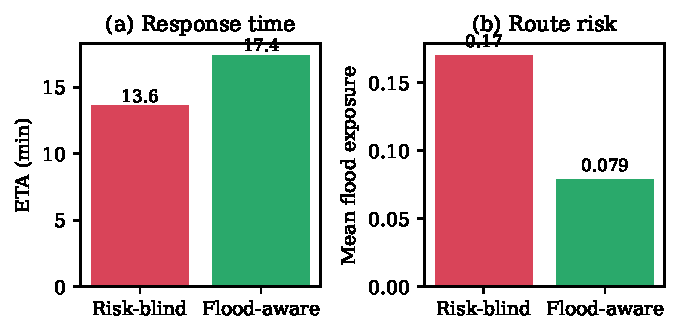
\includegraphics[width=0.8\linewidth]{figures/routing_exposure.pdf}
\caption{Risk-blind versus flood-aware routing for the representative pair:
response time and mean route exposure.}
\label{fig:routing_exposure}
\end{figure}

\subsection{Sensitivity of the routing constants}
\label{sec:res-sensitivity}

Figure~\ref{fig:sensitivity} and Table~\ref{tab:sensitivity} report the full
$7\times7$ sweep of $(\kappa,\tau)$, recomputing all 49 hospital-incident pairs
in each of the 49 cells.

\paragraph{Correcting for survivorship} A naive reading of this sweep is
actively misleading, and the correction matters enough to state before the
results. At $\tau\le0.50$, 29 of the 49 pairs are severed, so a cell mean taken
over "whatever routed" is computed on the 20 survivors, which are systematically
the short inland pairs that avoid the river crossings. Compared against a cell at
$\tau\ge0.65$ averaging over all 49, an aggressive threshold appears to
\emph{lower} exposure and \emph{shorten} detours when it has really just discarded
the hard cases. All statistics below and in
Figure~\ref{fig:sensitivity}(a)--(b) are therefore computed over the 20 pairs
routable in \emph{every} one of the 49 cells, so the comparison is like with
like; panel (c) reports the severed count, which is the quantity that legitimately
varies. The risk-blind baseline over that common subset is mean exposure 0.111
over \SI{5.57}{\minute}.

\paragraph{The penalty weight barely matters above $\kappa\approx6$}
At $\tau=0.60$ over the common subset, mean exposure changes by less than 1\%
between $\kappa=8$ and $\kappa=16$. Once the penalty is large enough that the
router prefers any available lower-risk alternative, increasing it changes
nothing, because the residual exposure lies on segments with no alternative.
$\kappa=8$ is defensible not because it is optimal but because the outcome is
indifferent to it across a wide neighbourhood.

\paragraph{The impassability threshold is a different kind of parameter}
Holding $\kappa=8$, severed pairs go 29 at $\tau\le0.50$, 7 at
$\tau\in\{0.55,0.60\}$, and 0 at $\tau\ge0.65$. That is a step function rather
than a gradient, because passability turns on a small number of critical crossing
edges whose risk values cluster tightly. The operating point sits one step above
a regime in which well over half the service pairs become unreachable.

Once survivorship is removed, the exposure spread across the eight cells
neighbouring the operating point falls from 15.9\% to 2.4\%, so the
\emph{exposure} outcome is far more stable than the uncorrected sweep suggested.
The consequential variation was never in exposure; it is in connectivity. The
conclusion is accordingly not that the parameters are stable, but that one of
them is immaterial while the other decides which parts of the city remain
reachable at all. $\tau$ should be set by policy on acceptable risk, informed by
panel (c), and calibrated locally against observed road closures rather than
inherited as a modelling convention.

\begin{figure}[t]
\centering

\includegraphics[width=\linewidth]{figures/sensitivity_sweep.pdf}
\caption{Sensitivity of the routing outcome to the penalty weight $\kappa$ and
impassability threshold $\tau$ at $T=0.70$. (a) Mean route exposure and
(b) mean detour, both over the 20 pairs routable in \emph{every} cell of the
sweep so that cells are compared like with like; (c) severed pairs, over all 49.
Vertical banding shows the outcome depends on $\tau$ far more than on $\kappa$;
the red box marks the operating point.}
\label{fig:sensitivity}
\end{figure}

\begin{table*}[!t]
\centering\footnotesize
\caption{Sensitivity sweep, selected sections. Exposure and detour are computed
over the 20 pairs routable in \emph{every} cell of the sweep, so columns are
comparable; the severed count is over all 49. Risk-blind baseline on that common
subset: mean exposure 0.111 over \SI{5.57}{\minute}.}
\label{tab:sensitivity}
\small
\begin{tabular}{@{}rrr@{\qquad\qquad}rrrr@{}}
\toprule
\multicolumn{3}{c}{\textbf{$\tau = 0.60$ fixed}} &
\multicolumn{4}{c}{\textbf{$\kappa = 8$ fixed}} \\
\cmidrule(lr){1-3}\cmidrule(lr){4-7}
$\boldsymbol{\kappa}$ & \textbf{Exposure} & \textbf{Detour (min)} &
$\boldsymbol{\tau}$ & \textbf{Exposure} & \textbf{Detour (min)} & \textbf{Severed} \\
\midrule
2  & 0.0909 & 0.14 & 0.45 & 0.0741 & 0.56 & 29 \\
4  & 0.0871 & 0.18 & 0.50 & 0.0741 & 0.56 & 29 \\
6  & 0.0791 & 0.32 & 0.55 & 0.0787 & 0.37 & 7 \\
\textbf{8}  & \textbf{0.0797} & \textbf{0.33} & \textbf{0.60} & \textbf{0.0797} & \textbf{0.33} & \textbf{7} \\
10 & 0.0788 & 0.38 & 0.65 & 0.0797 & 0.33 & 0 \\
12 & 0.0769 & 0.45 & 0.70 & 0.0797 & 0.33 & 0 \\
16 & 0.0769 & 0.45 & 0.75 & 0.0797 & 0.33 & 0 \\
\bottomrule
\end{tabular}
\end{table*}

\subsection{Dijkstra versus A$^\ast$: a multi-query benchmark}
\label{sec:res-algo}

Table~\ref{tab:algo} and Figure~\ref{fig:routing_benchmark} report all 42
reachable hospital-incident pairs under the May 2025 trigger. Seven of the 49
originate from one hospital whose road approaches are entirely severed at this
trigger, itself a legitimate finding and not a data problem.

Across the full set of 42 pairs the two searches agreed exactly, matching on both
the recovered path and its cost in every case, which is the empirical consequence
of the verified admissibility of Equation~\eqref{eq:heuristic}. A$^\ast$ settled
strictly fewer nodes on all 42, with a median reduction of 31.1\%.

Two nuances only a multi-query benchmark exposes. First, the benefit is highly
uneven: the reduction ranges from 52.9\% down to 0.03\%. The worst case is the
Bunder incident on the tidal margin, where the road network's connectivity forces
a circuitous approach and straight-line distance is a very poor proxy for road
distance, making the admissible heuristic nearly uninformative (\num{7991} versus
\num{7989} nodes). Second, and running against the node-count result, A$^\ast$ is
faster in wall-clock time on only 25 of 42 pairs, with a higher mean
(\SI{10.41}{\milli\second} versus \SI{8.70}{\milli\second}). Evaluating the
haversine heuristic at every expansion costs more in interpreted Python than the
expansions it saves. We report this without adjustment: it is a genuine property
of a search-transparent reference implementation, and it would reverse in a
compiled router, but presenting only the node-count result would misrepresent
what was measured.

\begin{table*}[!t]
\centering\footnotesize
\caption{Dijkstra versus A$^\ast$ across 42 reachable hospital-incident pairs at
$T=0.70$.}
\label{tab:algo}
\small
\begin{tabular}{@{}lrr@{}}
\toprule
\textbf{Metric} & \textbf{Dijkstra} & \textbf{A}$^\ast$ \\
\midrule
Mean nodes explored & \num{3349} & \num{2933} \\
Median per-pair node reduction & \multicolumn{2}{c}{31.1\%} \\
Range of per-pair reduction & \multicolumn{2}{c}{0.03\% -- 52.9\%} \\
Pairs where A$^\ast$ explores fewer & \multicolumn{2}{c}{42 / 42} \\
Mean wall time & \SI{8.70}{\milli\second} & \SI{10.41}{\milli\second} \\
Pairs where A$^\ast$ is faster & \multicolumn{2}{c}{25 / 42} \\
Identical optimal path and cost & \multicolumn{2}{c}{42 / 42} \\
\bottomrule
\end{tabular}
\end{table*}

\begin{figure}[t]
\centering
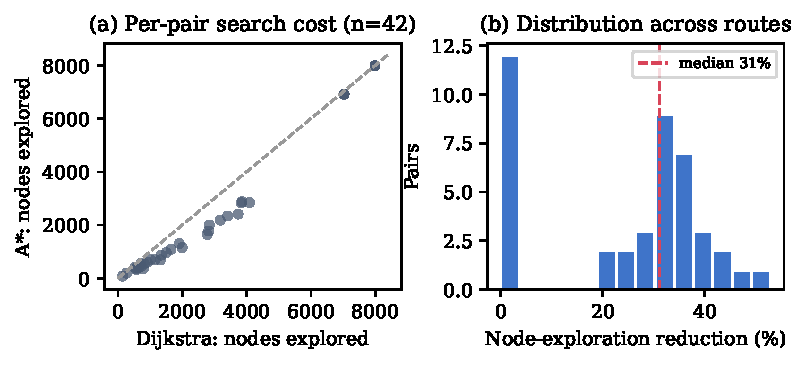
\includegraphics[width=\linewidth]{figures/routing_benchmark.pdf}
\caption{(a) Per-pair search cost; points below the diagonal indicate A$^\ast$
explored fewer nodes. (b) Distribution of per-pair node-exploration reduction,
median 31.1\%.}
\label{fig:routing_benchmark}
\end{figure}

\subsection{Hybrid quantum dispatch}
\label{sec:res-qaoa}

The QUBO ground state matches the Hungarian optimum exactly in both scenarios:
\SI{20.900}{\minute} for dry conditions and \SI{22.130}{\minute} under the
May 2025 trigger. Table~\ref{tab:qaoa} and Figure~\ref{fig:qaoa} report the depth
study over five seeds.

Averaged over seeds, the approximation ratio improves with depth in both
scenarios, from $0.8824\pm0.0022$ to $0.9248\pm0.0148$ (dry) and
$0.8695\pm0.0050$ to $0.9209\pm0.0059$ (flood). The improvement is real but
saturates: essentially all of it is realised by $p=3$, and the $p=4\to5$
increments ($+0.0010$ dry, $+0.0011$ flood) are an order of magnitude smaller
than the corresponding seed-to-seed standard deviations, so we do not claim a
demonstrated increase beyond $p\approx3$--$4$. Even the ordering that does hold
is a multi-seed result: individual seeds produce non-monotone sequences, because
COBYLA is a local optimiser on a non-convex landscape and the INTERP warm start
does not guarantee improvement.

The probability of directly sampling the optimum rises from roughly $2\%$ at
$p=1$ to a peak near $7\%$ at $p=4$, between $9\times$ and $40\times$ the uniform
random baseline of $1/512$, and is plainly \emph{not} monotone: it falls at $p=5$
in both scenarios. With standard deviations comparable to the means at higher
depths, it should be read as a trend with a plateau, not a specification.

The optimal assignment is identical under dry and flood conditions. We had
expected re-allocation and did not observe it: at this fleet size and geometry,
flooding changes travel times enough to alter route \emph{shape}
(Section~\ref{sec:res-routing}) but not enough to alter the assignment's relative
ordering. The finding is reported as observed.

We state plainly that at $n=3$ the Hungarian algorithm is exact and effectively
instantaneous, while the QAOA simulation takes seconds and returns the optimum
only probabilistically. This layer is a feasibility demonstration of the
QUBO/QAOA formulation on a real risk-aware cost matrix, not a claim of quantum
advantage. Its value is that the encoding, the constraint penalties and the
verification path are in place should problem sizes and hardware make the
question live.

\begin{table*}[!t]
\centering\footnotesize
\caption{QAOA depth study, 9 qubits, exact statevector, mean $\pm$ s.d.\ over
5 seeds with INTERP warm starting. ``Lift'' is mean optimum-sampling probability
relative to the uniform baseline $1/2^9$.}
\label{tab:qaoa}
\small
\begin{tabular}{@{}rlrrrrr@{}}
\toprule
$\boldsymbol{p}$ & \textbf{Scenario} & \textbf{Params} &
\textbf{Approx.\ ratio} & \textbf{Best} & \textbf{P(optimum)} & \textbf{Lift} \\
\midrule
1 & Dry & 2 & $0.8824\pm0.0022$ & 0.8864 & $0.0226\pm0.0026$ & $11.6\times$ \\
2 & Dry & 4 & $0.9116\pm0.0067$ & 0.9209 & $0.0503\pm0.0125$ & $25.8\times$ \\
3 & Dry & 6 & $0.9222\pm0.0059$ & 0.9301 & $0.0620\pm0.0120$ & $31.7\times$ \\
4 & Dry & 8 & $0.9238\pm0.0074$ & 0.9349 & $0.0704\pm0.0263$ & $36.0\times$ \\
5 & Dry & 10 & $0.9248\pm0.0148$ & 0.9414 & $0.0531\pm0.0231$ & $27.2\times$ \\
\midrule
1 & Flood & 2 & $0.8695\pm0.0050$ & 0.8738 & $0.0168\pm0.0074$ & $8.6\times$ \\
2 & Flood & 4 & $0.8976\pm0.0107$ & 0.9138 & $0.0323\pm0.0163$ & $16.5\times$ \\
3 & Flood & 6 & $0.9179\pm0.0071$ & 0.9283 & $0.0529\pm0.0154$ & $27.1\times$ \\
4 & Flood & 8 & $0.9198\pm0.0042$ & 0.9268 & $0.0781\pm0.0429$ & $40.0\times$ \\
5 & Flood & 10 & $0.9209\pm0.0059$ & 0.9312 & $0.0697\pm0.0391$ & $35.7\times$ \\
\bottomrule
\end{tabular}
\end{table*}

\begin{figure*}[!t]
\centering

\includegraphics[width=\linewidth]{figures/qaoa_depth.pdf}
\caption{QAOA depth study over five seeds. (a) Approximation ratio, mean
$\pm$ 1 s.d.; the trend is monotone in the mean for both scenarios.
(b) Optimum-sampling probability against the uniform baseline over $2^9$ states.}
\label{fig:qaoa}
\end{figure*}

\subsection{Limitations}
\label{sec:limitations}
\begin{itemize}
\item \textbf{The impassability threshold is a heuristic, not hydraulics.}
      $\tau$ marks a susceptibility level, not a fordable water depth, and the
      sweep shows the routing outcome turns on it.
\item \textbf{Travel times are free-flow.} No traffic model, no signal delay and
      no weather effect on speed is included, so absolute response times are
      optimistic even where the relative comparison holds.
\item \textbf{The wall-clock comparison reflects an interpreted implementation}
      chosen for search transparency; a compiled router would convert the
      node-count advantage into time saved.
\item \textbf{The quantum layer is a feasibility demonstration} at $3\times3$.
      The Hungarian algorithm is optimal and effectively instantaneous at this
      size, and no quantum advantage is claimed.
\item \textbf{Dispatch is single-shot.} Vehicles are assigned once, with no
      queueing, no re-routing in flight and no fleet dynamics.
\end{itemize}

\subsection{Comparison with prior work}
Risk-weighted routing under flooding is established~\cite{zhang2019,yin2016},
and QAOA has been applied to vehicle routing and assignment at comparable
scale~\cite{farhi2014,lucas2014,zhou2020}. What is different here is the
provenance of the weights: the per-edge risk is not an assumed inundation
scenario but a SAR-grounded, calibration-audited surface carried over from
Part~I, and the cost constants that convert it into a route are swept rather
than asserted.
\section{Conclusions}
This paper took the risk surface built in Part~I into the response layer and
measured what it buys.

\begin{enumerate}
\item \textbf{Flood-aware routing removes a third of mean route exposure} across
      all hospital-incident pairs, for a detour of a few minutes on a
      representative route. The gain is real but bounded by the network: both
      the risk-blind and the flood-aware route must cross the same small number
      of river crossings.
\item \textbf{The two cost constants are not equally consequential.} The penalty
      weight is immaterial above $\kappa\approx6$; the impassability threshold
      governs a step change in connectivity and must therefore be set by policy
      on acceptable risk, not by convention. Comparing sweep cells naively
      invites survivorship bias, because an aggressive threshold silently drops
      the hardest pairs, so cells are compared on the subset routable
      everywhere.
\item \textbf{Search-transparent benchmarking exposes a trade single examples
      hide.} A$^\ast$ returned the identical optimal path on all 42 pairs and
      explored a median 31.1\% fewer nodes, yet was faster in wall-clock time on
      only 25 of them, because heuristic evaluation costs more in interpreted
      Python than the expansions it avoids.
\item \textbf{The QUBO/QAOA dispatch layer reproduces the Hungarian optimum
      exactly} and improves with circuit depth over five seeds, at a problem
      size where it offers no advantage. We report it as a feasibility result
      and nothing more.
\end{enumerate}

Future work follows from the limitations of both parts. A calibrated depth
regression would replace the heuristic impassability threshold with a hydraulic
criterion and make $\tau$ a physical quantity. A spatially resolved rainfall
field would make the trigger genuinely spatiotemporal. A compiled routing
implementation would isolate the algorithmic advantage of A$^\ast$ from
interpreter overhead, and executing the QAOA circuits on physical hardware would
characterise the noise behaviour exact simulation cannot.

\balance
\begin{thebibliography}{99}
\setlength{\itemsep}{1pt}

\bibitem[Companion(2026a)]{parti} Authors. Spatiotemporal flood risk modelling under a single-orbit SAR constraint, Part~I: Confound-controlled susceptibility and a three-stage validation ladder. \emph{Companion paper, submitted}.

\bibitem[Zhang et al.(2019)]{zhang2019}
N.~Zhang, H.~Alipour.
Multi-scale analysis of the impact of flooding on the urban road network.
\emph{Transportation Research Part D}, 77:279--293, 2019.

\bibitem[Yin et al.(2016)]{yin2016}
J.~Yin, D.~Yu, Z.~Yin, M.~Liu, Q.~He.
Evaluating the impact and risk of pluvial flash flood on intra-urban road network.
\emph{Journal of Hydrology}, 537:138--145, 2016.

\bibitem[Hart et al.(1968)]{hart1968}
P.~E.~Hart, N.~J.~Nilsson, B.~Raphael.
A formal basis for the heuristic determination of minimum cost paths.
\emph{IEEE Transactions on Systems Science and Cybernetics}, 4(2):100--107, 1968.

\bibitem[Dijkstra(1959)]{dijkstra1959}
E.~W.~Dijkstra.
A note on two problems in connexion with graphs.
\emph{Numerische Mathematik}, 1:269--271, 1959.

\bibitem[Church and ReVelle(1974)]{church1974}
R.~Church, C.~ReVelle.
The maximal covering location problem.
\emph{Papers in Regional Science}, 32(1):101--118, 1974.
\href{https://doi.org/10.1111/j.1435-5597.1974.tb00902.x}{doi:10.1111/j.1435-5597.1974.tb00902.x}.

\bibitem[Brotcorne et al.(2003)]{brotcorne2003}
L.~Brotcorne, G.~Laporte, F.~Semet.
Ambulance location and relocation models.
\emph{European Journal of Operational Research}, 147(3):451--463, 2003.
\href{https://doi.org/10.1016/S0377-2217(02)00364-8}{doi:10.1016/S0377-2217(02)00364-8}.

\bibitem[Kuhn(1955)]{kuhn1955}
H.~W.~Kuhn.
The Hungarian method for the assignment problem.
\emph{Naval Research Logistics Quarterly}, 2(1--2):83--97, 1955.

\bibitem[Farhi et al.(2014)]{farhi2014}
E.~Farhi, J.~Goldstone, S.~Gutmann.
A quantum approximate optimization algorithm.
\emph{arXiv:1411.4028}, 2014.

\bibitem[Lucas(2014)]{lucas2014}
A.~Lucas. Ising formulations of many NP problems.
\emph{Frontiers in Physics}, 2:5, 2014.

\bibitem[Zhou et al.(2020)]{zhou2020}
L.~Zhou, S.-T.~Wang, S.~Choi, H.~Pichler, M.~D.~Lukin.
Quantum approximate optimization algorithm: performance, mechanism, and
implementation on near-term devices.
\emph{Physical Review X}, 10:021067, 2020.

\bibitem[McClean et al.(2018)]{mcclean2018}
J.~R.~McClean, S.~Boixo, V.~N.~Smelyanskiy, R.~Babbush, H.~Neven.
Barren plateaus in quantum neural network training landscapes.
\emph{Nature Communications}, 9:4812, 2018.

\bibitem[Boeing(2017)]{boeing2017}
G.~Boeing.
OSMnx: New methods for acquiring, constructing, analyzing, and visualizing
complex street networks.
\emph{Computers, Environment and Urban Systems}, 65:126--139, 2017.
\href{https://doi.org/10.1016/j.compenvurbsys.2017.05.004}{doi:10.1016/j.compenvurbsys.2017.05.004}.

\bibitem[Powell(1994)]{powell1994}
M.~J.~D.~Powell.
A direct search optimization method that models the objective and constraint
functions by linear interpolation.
In \emph{Advances in Optimization and Numerical Analysis}, pages 51--67.
Springer, 1994.
\href{https://doi.org/10.1007/978-94-015-8330-5_4}{doi:10.1007/978-94-015-8330-5\_4}.

\bibitem[Pedregosa et al.(2011)]{pedregosa2011}
F.~Pedregosa, G.~Varoquaux, A.~Gramfort, et al.
Scikit-learn: Machine learning in Python.
\emph{Journal of Machine Learning Research}, 12:2825--2830, 2011.

\bibitem[Chen and Guestrin(2016)]{chen2016}
T.~Chen, C.~Guestrin.
XGBoost: A scalable tree boosting system.
In \emph{Proc.\ 22nd ACM SIGKDD}, pages 785--794, 2016.

\bibitem[Lundberg and Lee(2017)]{lundberg2017}
S.~M.~Lundberg, S.-I.~Lee.
A unified approach to interpreting model predictions.
In \emph{Advances in Neural Information Processing Systems 30}, 2017.

\bibitem[Harris et al.(2020)]{harris2020}
C.~R.~Harris, K.~J.~Millman, S.~J.~van~der~Walt, et al.
Array programming with NumPy.
\emph{Nature}, 585:357--362, 2020.
\href{https://doi.org/10.1038/s41586-020-2649-2}{doi:10.1038/s41586-020-2649-2}.

\bibitem[Virtanen et al.(2020)]{virtanen2020}
P.~Virtanen, R.~Gommers, T.~E.~Oliphant, et al.
SciPy 1.0: Fundamental algorithms for scientific computing in Python.
\emph{Nature Methods}, 17:261--272, 2020.
\href{https://doi.org/10.1038/s41592-019-0686-2}{doi:10.1038/s41592-019-0686-2}.

\bibitem[Hunter(2007)]{hunter2007}
J.~D.~Hunter.
Matplotlib: A 2D graphics environment.
\emph{Computing in Science \& Engineering}, 9(3):90--95, 2007.
\href{https://doi.org/10.1109/MCSE.2007.55}{doi:10.1109/MCSE.2007.55}.

\end{thebibliography}

\end{document}
